\documentclass[11pt, twoside]{report}

\usepackage{fontspec}
\usepackage[utf8]{inputenc}
\usepackage[bitstream-charter]{mathdesign}
\usepackage{bbding}
\usepackage{ragged2e}
\usepackage{parskip}
\usepackage{enumitem}
\usepackage{titlesec}
\usepackage{paracol}
\usepackage{mdframed}
\usepackage[margin=1in]{geometry}

\usepackage[autocompile]{gregoriotex}

\titleformat{\chapter}[block]{\huge\scshape\filcenter}{}{1em}{}
\titleformat{\section}[block]{\Large\bfseries\filcenter}{}{1em}{}

\mdfsetup{skipabove=\topskip, skipbelow=\topskip}

\newcommand{\rubric}[1]{
	\switchcolumn[0] {
		\itshape
		#1
	}
}

\newcommand{\latinenglish}[2]{
	\switchcolumn[0]* {
		#1
	}
	\switchcolumn[1] {
		\itshape\small
		#2
	}
}

\newcommand{\latinenglishequal}[2]{
	\switchcolumn[0]* {
		#1
	}
	\switchcolumn[1] {
		\itshape
		#2
	}
}

\newenvironment{latinenglishsection}
	{\columnratio{.7, .3} \begin{paracol}{2}}
	{\end{paracol}}

\newenvironment{latinenglishequalsection}
	{\columnratio{.5, .5}\begin{paracol}{2}}
	{\end{paracol}}

\setlength{\columnseprule}{0.4pt}

\newcommand{\heading}[1]{
	\begin{leftcolumn}
		#1
	\end{leftcolumn}
}

\newcommand{\spanning}[1]{
	\switchcolumn*[#1]
}

\newenvironment{verses}[1]
	{\begin{flushleft} \begin{enumerate}[leftmargin=*] \setcounter{enumi}{#1}}
	{\end{enumerate} \end{flushleft}}

\newenvironment{versicles}{\par\leavevmode\parskip=0pt}{}

\newenvironment{collect}
{
	\leavevmode
	\parindent=1em
	\parskip=0pt
	\noindent Orémus.\par
}{}

\newenvironment{optionbox}
{
	\switchcolumn[0]
	\begin{mdframed}
%	\begin{minipage}{0.8\linewidth}
}{
%	\end{minipage}
	\end{mdframed}
}

\newcommand{\optionrule}{
	\begin{center}
	\rule{0.5\linewidth}{0.6pt}
	\end{center}
}

\newenvironment{optionruled}
{
	\optionrule
}
{
	\optionrule
}

% for use inside the collect environment
\newcommand{\Amen}{\par\noindent \Rbar. Amen.}

\begin{document}

%\title{Compline of The Blessed Virgin Mary}
%\date{ }

\vspace*{2cm}

\begin{center}
	\textbf{\Huge None of the Blessed Virgin Mary}\\
	{\LARGE According to the Washtenaw Use}
\end{center}

\vspace*{1cm}
%\maketitle

%\begin{figure}[h!]
	%\centering
%\end{figure}

\begin{center}
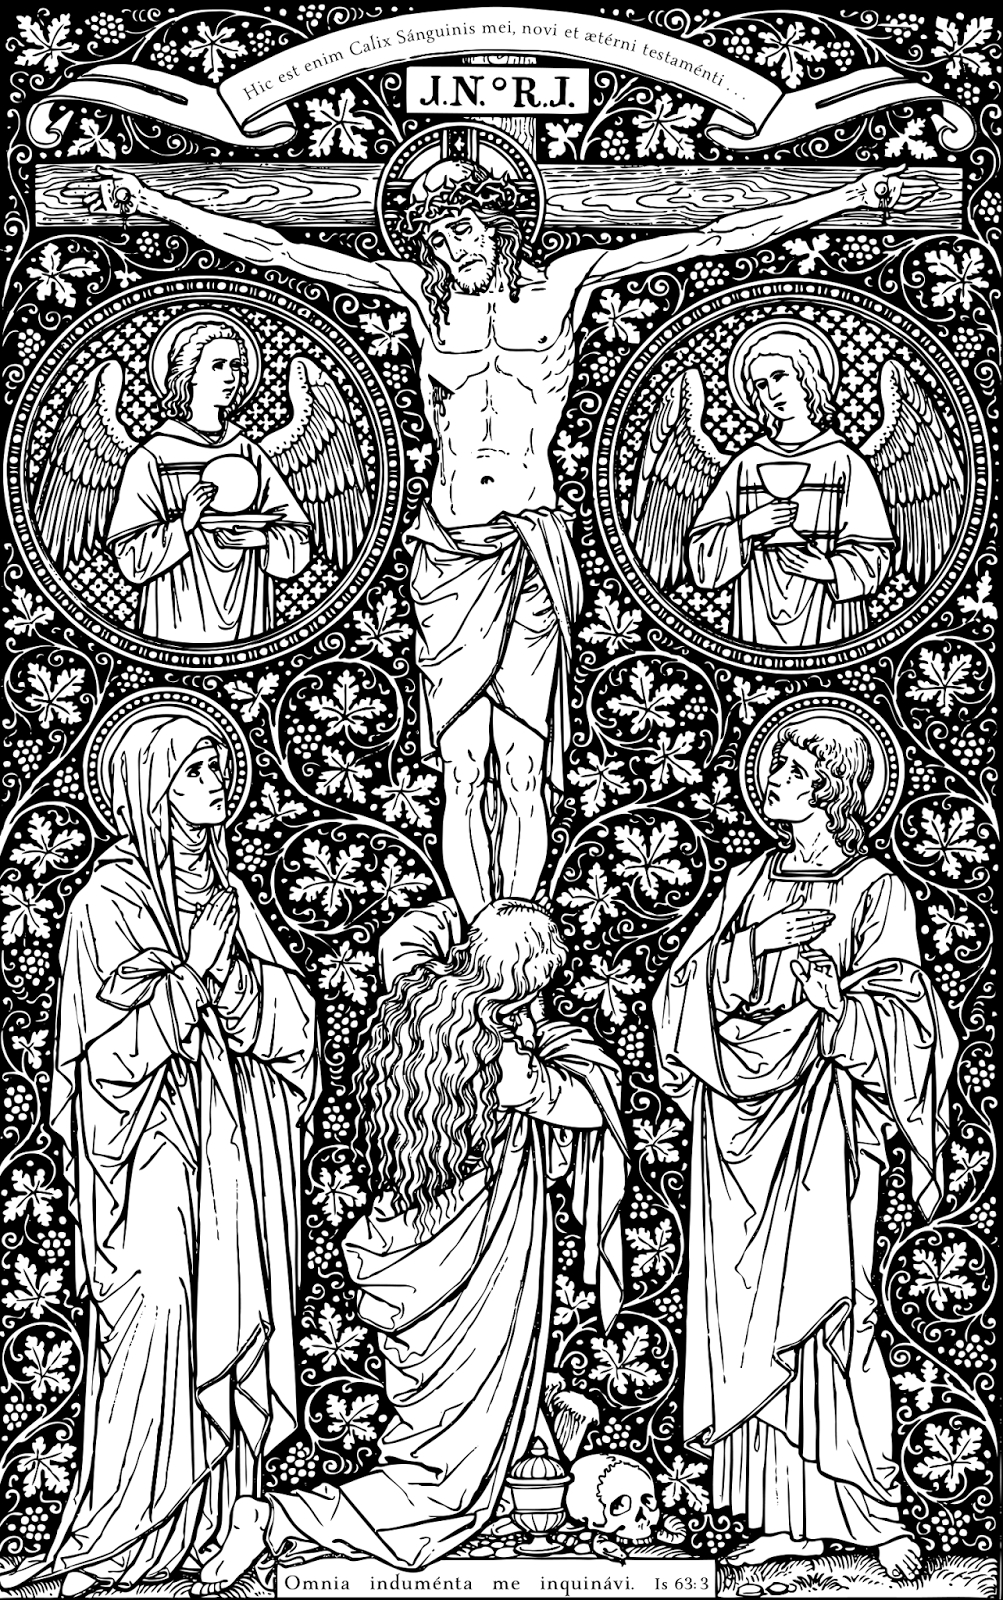
\includegraphics[width=0.5\textwidth]{ChristCrucified}
\end{center}

\hspace{0pt}
\vfill

\pagebreak

\vspace*{7.5cm}
``At the hour of \textit{None}, Our Lord Jesus Christ cired, and gave out His soul by death. The same hour, a knight opened Our Lord's side with a spear, and smote through His Heart, whereout came water to our baptism, and blood to our redemption.'' (Paraphrased from the \textit{Mirror of Our Lady.}) O most Blessed Virgin, you stood by your son, sharing in the pain of His Passion, pray that we would never weight lightly the redemption that He won for us by His wounds on the rood. Amen.
\vfill

\pagebreak

\chapter*{Before None}

\section*{Preparatory Prayers}

\textit{ All kneel and pray silently. As you say the prayer \textnormal{Aperi, Domine}, make the sign of the cross with your thumb first over your lips, and then over your heart.}

\begin{latinenglishequalsection}

\latinenglishequal{
	Áperi, {\color{red}\maltese}\ Dómine, os meum ad benedicéndum\linebreak nomen sanctum tuum:
	{\color{red}\maltese}\ munda quoque cor meum ab ómnibus vanis, pervérsis et aliénis cogitatiónibus;
	intelléctum illúmina, afféctum inflámma, ut digne, atténte ac devóte hoc Offícium beátæ Vírginis Maríæ recitáre váleam,
	et exaudíri mérear ante conspéctum divínæ Majestátis tuæ.
	Per Christum Dóminum nostrum. 
	Amen.
}{
	Open, {\color{red}\maltese}\ O Lord, my mouth to bless Thy holy Name; {\color{red}\maltese}\ cleanse also my heart from all vain, evil, and wandering thoughts; enlighten my understanding and kindle my affections; that I may worthily, attentively, and devoutly say this Office of the Blessed Virgin Mary, and so merit to be heard before the presence of Thy divine Majesty.  Through Christ our Lord.  Amen.
}

\latinenglishequal{
	Domine, in unióne illíus divínæ intentiónis, qua ipse in terris laudes Deo persolvísti, has tibi Horas persólvo.
}{
	O Lord, in union with that divine intention wherewith thou, whilst here on earth, didst render praises unto God, I desire to offer this my Office of prayer unto thee.
}

\latinenglishequal{
	Ave María, grátia plena, Dóminus tecum. Benedíc\-ta tu in muliéribus, et benedíctus fructus ventris tui, Jesus.
 Sancta María, Mater Dei, ora pro nobis peccatóribus, nunc et in hora mortis nostræ. Amen.
 }{
 	Hail Mary, full of grace, the Lord is with thee. Blessed art thou among women, and blessed is the fruit of thy womb, Jesus.
 Holy Mary, Mother of God, pray for us sinners, now and at the hour of our death. Amen.
 }
 
 \end{latinenglishequalsection}
 
\chapter*{None}

\begin{latinenglishsection}

\heading{\section*{Invitatory}}

\rubric{\color{red}All make the Sign of the Cross as the Officiant says the ``Deus in Adjutorium''. All continue together with the entire ``Gloria Patri'' after the response: }

\latinenglish{
	\gresetinitiallines{1}
	\gregorioscore{deus_in_adjutorium_minor}
}{
	O God, come to my assistance.
		
	O Lord, make haste to help me.
	
	Glory be to the Father, and to the Son, and to the Holy Spirit,
	as it was in the beginning, is now, and ever shall be, world without end. Amen.
	
	Alleluia.
}

\rubric{\color{red}From Septuagesima until Easter, \textnormal{Alleluia} is replaced with:}

\latinenglish{
	\gresetinitiallines{0}
	\gabcsnippet{
	(c3)Lau(h)s ti(h)bi(h) Dó(h)mi(h)ne(h), Re(h)x æ(h)té(h)rnæ(i) gló(h)ri(h)æ.(g) (::)
	}
}{
	Praise to thee, O Lord, King of everlasting glory.
}

\end{latinenglishsection}

\vfill\pagebreak

\begin{latinenglishsection}

\heading{\section*{Hymn}}

\latinenglish{
	\gresetinitiallines{0}
	\gregorioscore{memento_rerum_conditor}
}{
	1. Remember, Make of all things, 
	That once the form of our flesh, 
	From the Virgin's sacred womb, 
	Being born, Thou didst assume.
	
	2. Mary, Mother of grace, 
	Sweet parent of clemency, 
	Thou protect us from the enemy, 
	And receive us at the hour of death.
	
	3. Jesus, to Thee be glory, 
	Who wast born of the Virgin, 
	With the Father, and the loving Spirit, 
	Unto sempiternal ages. Amen.
}

\rubric{\color{red} For `Throughout the Year', \underline{see page 6}.}
\rubric{\color{red} For `Advent', \underline{see page 9}.}
\rubric{\color{red} For `Christmastide', \underline{see page 12}.}

\end{latinenglishsection}

\vfill\pagebreak

\section*{THROUGHOUT THE YEAR}

\begin{latinenglishsection}

% Psalm cix: In convertendo (with antiphon)

\heading{\section*{Psalm 125}}

\rubric{\color{red}The Cantor intones the antiphon and leads the first Psalm verse to the star (*). All sit, while the Cantor's side finishes the first verse together. The Officiants side then says the second Psalm verse, with each side alternating thereafter. The remaining Psalms are intoned up to the asterisk by the Cantor, repeating the pattern of sitting and standing until the antiphon is said in full at the very end.}

\latinenglish{
	\gresetinitiallines{1}
	\gregorioscore{pulchra_es_et_decora_intonation}
}{
	Thou art fair and comely...
}

\latinenglish{
	\gresetinitiallines{0}
	\gregorioscore{psalm_125_1_1g2}
	
	\begin{verses}{1}
	
	\item Tunc replétum est gáudi\textbf{o} os \textbf{nos}trum:~* et lingua nostra exsul\textit{ta}\textit{ti}\textbf{ó}ne.

	\item Tunc dicent \textbf{in}ter \textbf{Gen}tes:~* Magnificávit Dóminus fáce\textit{re} \textit{cum} \textbf{e}is.
	
	\item Magnificávit Dóminus fáce\textbf{re} no\textbf{bís}cum:~* facti su\textit{mus} \textit{læ}\textbf{tán}tes.
	
	\item Convérte, Dómine, captivi\textbf{tá}tem \textbf{nos}tram,~* sicut tor\textit{rens} \textit{in} \textbf{aus}tro.
	
	\item Qui sémi\textbf{nant} in \textbf{lá}crimis,~* in exsultati\textit{ó}\textit{ne} \textbf{me}tent.
	
	\item Eúntes \textbf{i}bant et \textbf{fle}bant,~* mitténtes sé\textit{mi}\textit{na} \textbf{su}a.
	
	\item Veniéntes autem vénient cum exsul\textbf{ta}ti\textbf{ó}ne,~* {\color{red}\textit{(stand)}} portántes maní\textit{pu}\textit{los} \textbf{su}os.
	
	\item {\color{red}\textit{(bow)}} Glória \textbf{Pa}tri, et \textbf{Fí}lio,~* et Spirí\textit{tu}\textit{i} \textbf{Sanc}to.
	
	\item {\color{red}\textit{(rise)}} Sicut erat in princípio, et \textbf{nunc}, et \textbf{sem}per,~* et in s\'{\ae}cula sæcu\textit{ló}\textit{rum}. \textbf{A}men.
	
	\end{verses}
}{
	1. When the Lord turned again the captivity of Sion:
	we became like men that are comforted.
	
	2. Then was our mouth filled with gladness:
	and our tongue with joy.
	
	3. Then shall they say among the gentiles:
	The Lord hath done great things for them.
	
	4. The Lord hath done great things for us:
	we are become very joyful.
	
	5. Turn again our captivity, O Lord:
	as a river in the south.
	
	6. They that sow in tears:
	shall reap in joy.
	
	7. Going on their way they went and wept:
	scattering their seed.
	
	8. But returning they shall come with joyfulness:
	bringing their sheaves with them.
	
	9. Glory be to the Father, and to the Son, and to the Holy Spirit:
	As it was in the beginning, is now, and ever shall be, world without end. Amen.
}

\end{latinenglishsection}

\vfill\pagebreak

\begin{latinenglishsection}

\heading{\section*{Psalm 126}}

\latinenglish{
	\gresetinitiallines{0}
	\gregorioscore{psalm_126_1_1g2}
	
	\begin{verses}{1}
	
	\item Nisi Dóminus custodíerit \textbf{ci}vi\textbf{tá}tem,~* frustra vígilat qui cus\textit{tó}\textit{dit} \textbf{e}am.

	\item Vanum est vobis ante \textbf{lu}cem \textbf{súr}gere:~* súrgite postquam sedéritis, qui manducátis pa\textit{nem} \textit{do}\textbf{ló}ris.
	
	\item Cum déderit diléctis \textbf{su}is \textbf{som}num:~* ecce heréditas Dómini fílii: merces, \textit{fruc}\textit{tus} \textbf{ven}tris.
	
	\item Sicut sagíttæ in \textbf{ma}nu pot\textbf{én}tis:~* ita fílii \textit{ex}\textit{cus}\textbf{só}rum.
	
	\item Beátus vir qui implévit desidérium \textbf{su}um ex \textbf{ip}sis:~* {\color{red}\textit{(stand)}} non confundétur cum loquétur inimícis su\textit{is} \textit{in} \textbf{por}ta.
	
	\item {\color{red}\textit{(bow)}} Glória \textbf{Pa}tri, et \textbf{Fí}lio,~* et Spirí\textit{tu}\textit{i} \textbf{Sanc}to.
	
	\item {\color{red}\textit{(rise)}} Sicut erat in princípio, et \textbf{nunc}, et \textbf{sem}per,~* et in s\'{\ae}cula sæcu\textit{ló}\textit{rum}. \textbf{A}men.
	
	\end{verses}
}{
	1. Unless the Lord build the house:
	they labour in vain that build it.
	
	2. Unless the Lord keep the city:
	he watcheth in vain that keepeth it.
	
	3. In vain ye rise before the light:
	rise not till ye have rest, O ye that eat the bread of sorrow.
	
	4. When he hath given sleep to his beloved:
	lo, children are an heritage from the Lord, and the fruit of the womb a reward.
	
	5. Like as arrows in the hand of the mighty one:
	so are the children of those who have been cast out.
	
	6. Blessed is the man whose desire is satisfied with them:
	he shall not be confoundd, when he speaketh with his enemies in the gate.
	
	7. Glory be to the Father, and to the Son, and to the Holy Spirit:
	As it was in the beginning, is now, and ever shall be, world without end. Amen.
}

%\end{latinenglishsection}

%\begin{latinenglishsection}

\heading{\section*{Psalm 127}}

\latinenglish{
	\gresetinitiallines{0}
	\gregorioscore{psalm_127_1_1g2}
	
	\begin{verses}{1}
	
	\item Labóres mánuum tuárum quia \textbf{man}du\textbf{cá}bis:~* beátus es, et bene \textit{ti}\textit{bi} \textbf{e}rit.

	\item Uxor tua sicut \textbf{vi}tis ab\textbf{ún}dans:~* in latéribus \textit{do}\textit{mus} \textbf{tu}æ.
	
	\item Fílii tui sicut novéllæ \textbf{o}li\textbf{vá}rum:~* in circúitu \textit{men}\textit{sæ} \textbf{tu}æ.
	
	\item Ecce sic benedi\textbf{cé}tur \textbf{ho}mo,~* qui \textit{ti}\textit{met} \textbf{Dó}minum.
	
	\item Benedícat tibi Dómi\textbf{nus} ex \textbf{Si}on:~* et vídeas bona Jerúsalem ómnibus diébus \textit{vi}\textit{tæ} \textbf{tu}æ.
	
	\item Et vídeas fílios fili\textbf{ó}rum tu\textbf{ó}rum:~* {\color{red}\textit{(stand)}} pacem \textit{su}\textit{per} \textbf{Is}raël.
	
	\item {\color{red}\textit{(bow)}} Glória \textbf{Pa}tri, et \textbf{Fí}lio,~* et Spirí\textit{tu}\textit{i} \textbf{Sanc}to.
	
	\item {\color{red}\textit{(rise)}} Sicut erat in princípio, et \textbf{nunc}, et \textbf{sem}per,~* et in s\'{\ae}cula sæcu\textit{ló}\textit{rum}. \textbf{A}men.
	
	\end{verses}
	
	\gresetinitiallines{1}
	\gregorioscore{pulchra_es_et_decora}
}{
	1. Blessed are all they that fear the Lord:
	that walk in his ways.
	
	2. For thou shalt eat the labours of thy hands:
	blessed art thou, and it shall be well with thee.
	
	3. Thy wife shall be as a fruitful vine: 
	on the walls of thy house.
	
	4. Thy children as olive plants:
	round about thy table.
	
	5. Behold, thus shall the man be blessed:
	that feareth the Lord.
	
	6. May the Lord bless thee out of Sion:
	and mayest thou see the good things of Jerusalem all the days of thy life.
	
	7. And mayest thou see thy children's children:
	peace upon Israel.
	
	8. Glory be to the Father, and to the Son, and to the Holy Spirit:
	As it was in the beginning, is now, and ever shall be, world without end. Amen.
	
	Thou art fair and comely, O daughter of Jerusalem: terrible as an army set in array.
}

\rubric{\color{red}Proceed to page 15.}

\end{latinenglishsection}

\vfill\pagebreak

\section*{ADVENT}

\begin{latinenglishsection}

% Psalm cix: In convertendo (with antiphon)

\heading{\section*{Psalm 125}}

\rubric{\color{red}The Cantor intones the antiphon and leads the first Psalm verse to the star (*). All sit, while the Cantor's side finishes the first verse together. The Officiants side then says the second Psalm verse, with each side alternating thereafter. The remaining Psalms are intoned up to the asterisk by the Cantor, repeating the pattern of sitting and standing until the antiphon is said in full at the very end.}

\latinenglish{
	\gresetinitiallines{1}
	\gregorioscore{ecce_ancilla_domini_intonation}
}{
	Behold the handmaid of the Lord...
}

\latinenglish{
	\gresetinitiallines{0}
	\gregorioscore{psalm_125_1_8G}
	
	\begin{verses}{1}
	
	\item Tunc replétum est gáudio os \textbf{nos}trum:~* et lingua nostra exsul\textit{ta}\textit{ti}\textbf{ó}ne.

	\item Tunc dicent inter \textbf{Gen}tes:~* Magnificávit Dóminus fáce\textit{re} \textit{cum} \textbf{e}is.
	
	\item Magnificávit Dóminus fácere no\textbf{bís}cum:~* facti su\textit{mus} \textit{læ}\textbf{tán}tes.
	
	\item Convérte, Dómine, captivitátem \textbf{nos}tram,~* sicut tor\textit{rens} \textit{in} \textbf{aus}tro.
	
	\item Qui séminant in \textbf{lá}crimis,~* in exsultati\textit{ó}\textit{ne} \textbf{me}tent.
	
	\item Eúntes ibant et \textbf{fle}bant,~* mitténtes sé\textit{mi}\textit{na} \textbf{su}a.
	
	\item Veniéntes autem vénient cum exsultati\textbf{ó}ne,~* {\color{red}\textit{(stand)}} portántes maní\textit{pu}\textit{los} \textbf{su}os.
	
	\item {\color{red}\textit{(bow)}} Glória Patri, et \textbf{Fí}lio,~* et Spirí\textit{tu}\textit{i} \textbf{Sanc}to.
	
	\item {\color{red}\textit{(rise)}} Sicut erat in princípio, et nunc, et \textbf{sem}per,~* et in s\'{\ae}cula sæcu\textit{ló}\textit{rum}. \textbf{A}men.
	
	\end{verses}
}{
	1. When the Lord turned again the captivity of Sion:
	we became like men that are comforted.
	
	2. Then was our mouth filled with gladness:
	and our tongue with joy.
	
	3. Then shall they say among the gentiles:
	The Lord hath done great things for them.
	
	4. The Lord hath done great things for us:
	we are become very joyful.
	
	5. Turn again our captivity, O Lord:
	as a river in the south.
	
	6. They that sow in tears:
	shall reap in joy.
	
	7. Going on their way they went and wept:
	scattering their seed.
	
	8. But returning they shall come with joyfulness:
	bringing their sheaves with them.
	
	9. Glory be to the Father, and to the Son, and to the Holy Spirit:
	As it was in the beginning, is now, and ever shall be, world without end. Amen.
}

\end{latinenglishsection}

\vfill\pagebreak

\begin{latinenglishsection}

\heading{\section*{Psalm 126}}

\latinenglish{
	\gresetinitiallines{0}
	\gregorioscore{psalm_126_1_8G}
	
	\begin{verses}{1}
	
	\item Nisi Dóminus custodíerit civi\textbf{tá}tem,~* frustra vígilat qui cus\textit{tó}\textit{dit} \textbf{e}am.

	\item Vanum est vobis ante lucem \textbf{súr}gere:~* súrgite postquam sedéritis, qui manducátis pa\textit{nem} \textit{do}\textbf{ló}ris.
	
	\item Cum déderit diléctis suis \textbf{som}num:~* ecce heréditas Dómini fílii: merces, \textit{fruc}\textit{tus} \textbf{ven}tris.
	
	\item Sicut sagíttæ in manu pot\textbf{én}tis:~* ita fílii \textit{ex}\textit{cus}\textbf{só}rum.
	
	\item Beátus vir qui implévit desidérium suum ex \textbf{ip}sis:~* {\color{red}\textit{(stand)}} non confundétur cum loquétur inimícis su\textit{is} \textit{in} \textbf{por}ta.
	
	\item {\color{red}\textit{(bow)}} Glória Patri, et \textbf{Fí}lio,~* et Spirí\textit{tu}\textit{i} \textbf{Sanc}to.
	
	\item {\color{red}\textit{(rise)}} Sicut erat in princípio, et nunc, et \textbf{sem}per,~* et in s\'{\ae}cula sæcu\textit{ló}\textit{rum}. \textbf{A}men.
	
	\end{verses}
}{
	1. Unless the Lord build the house:
	they labour in vain that build it.
	
	2. Unless the Lord keep the city:
	he watcheth in vain that keepeth it.
	
	3. In vain ye rise before the light:
	rise not till ye have rest, O ye that eat the bread of sorrow.
	
	4. When he hath given sleep to his beloved:
	lo, children are an heritage from the Lord, and the fruit of the womb a reward.
	
	5. Like as arrows in the hand of the mighty one:
	so are the children of those who have been cast out.
	
	6. Blessed is the man whose desire is satisfied with them:
	he shall not be confoundd, when he speaketh with his enemies in the gate.
	
	7. Glory be to the Father, and to the Son, and to the Holy Spirit:
	As it was in the beginning, is now, and ever shall be, world without end. Amen.
}

%\end{latinenglishsection}

%\begin{latinenglishsection}

\heading{\section*{Psalm 127}}

\latinenglish{
	\gresetinitiallines{0}
	\gregorioscore{psalm_127_1_8G}
	
	\begin{verses}{1}
	
	\item Labóres mánuum tuárum quia mandu\textbf{cá}bis:~* beátus es, et bene \textit{ti}\textit{bi} \textbf{e}rit.

	\item Uxor tua sicut vitis ab\textbf{ún}dans:~* in latéribus \textit{do}\textit{mus} \textbf{tu}æ.
	
	\item Fílii tui sicut novéllæ oli\textbf{vá}rum:~* in circúitu \textit{men}\textit{sæ} \textbf{tu}æ.
	
	\item Ecce sic benedicétur \textbf{ho}mo,~* qui \textit{ti}\textit{met} \textbf{Dó}minum.
	
	\item Benedícat tibi Dóminus ex \textbf{Si}on:~* et vídeas bona Jerúsalem ómnibus diébus \textit{vi}\textit{tæ} \textbf{tu}æ.
	
	\item Et vídeas fílios filiórum tu\textbf{ó}rum:~* {\color{red}\textit{(stand)}} pacem \textit{su}\textit{per} \textbf{Is}raël.
	
	\item {\color{red}\textit{(bow)}} Glória Patri, et \textbf{Fí}lio,~* et Spirí\textit{tu}\textit{i} \textbf{Sanc}to.
	
	\item {\color{red}\textit{(rise)}} Sicut erat in princípio, et nunc, et \textbf{sem}per,~* et in s\'{\ae}cula sæcu\textit{ló}\textit{rum}. \textbf{A}men.
	
	\end{verses}
	
	\gresetinitiallines{1}
	\gregorioscore{ecce_ancilla_domini}
}{
	1. Blessed are all they that fear the Lord:
	that walk in his ways.
	
	2. For thou shalt eat the labours of thy hands:
	blessed art thou, and it shall be well with thee.
	
	3. Thy wife shall be as a fruitful vine: 
	on the walls of thy house.
	
	4. Thy children as olive plants:
	round about thy table.
	
	5. Behold, thus shall the man be blessed:
	that feareth the Lord.
	
	6. May the Lord bless thee out of Sion:
	and mayest thou see the good things of Jerusalem all the days of thy life.
	
	7. And mayest thou see thy children's children:
	peace upon Israel.
	
	8. Glory be to the Father, and to the Son, and to the Holy Spirit:
	As it was in the beginning, is now, and ever shall be, world without end. Amen.
	
	Behold the handmaid of the Lord: be it done unto me according to thy word.
}

\rubric{\color{red}Proceed to page 15.}

\end{latinenglishsection}

\vfill\pagebreak

\section*{CHRISTMASTIDE}

\begin{latinenglishsection}

% Psalm cix: In convertendo (with antiphon)

\heading{\section*{Psalm 125}}

\rubric{\color{red}The Cantor intones the antiphon and leads the first Psalm verse to the star (*). All sit, while the Cantor's side finishes the first verse together. The Officiants side then says the second Psalm verse, with each side alternating thereafter. The remaining Psalms are intoned up to the asterisk by the Cantor, repeating the pattern of sitting and standing until the antiphon is said in full at the very end.}

\latinenglish{
	\gresetinitiallines{1}
	\gregorioscore{ecce_maria_genuit_intonation}
}{
	Behold, Mary hath borne us the Saviour...
}

\latinenglish{
	\gresetinitiallines{0}
	\gregorioscore{psalm_125_1_2D}
	
	\begin{verses}{1}
	
	\item Tunc replétum est gáudio os \textbf{nos}trum:~* et lingua nostra exsulta\textit{ti}\textbf{ó}ne.

	\item Tunc dicent inter \textbf{Gen}tes:~* Magnificávit Dóminus fácere \textit{cum} \textbf{e}is.
	
	\item Magnificávit Dóminus fácere no\textbf{bís}cum:~* facti sumus \textit{læ}\textbf{tán}tes.
	
	\item Convérte, Dómine, captivitátem \textbf{nos}tram,~* sicut torrens \textit{in} \textbf{aus}tro.
	
	\item Qui séminant in \textbf{lá}crimis,~* in exsultatió\textit{ne} \textbf{me}tent.
	
	\item Eúntes ibant et \textbf{fle}bant,~* mitténtes sémi\textit{na} \textbf{su}a.
	
	\item Veniéntes autem vénient cum exsultati\textbf{ó}ne,~* {\color{red}\textit{(stand)}} portántes manípu\textit{los} \textbf{su}os.
	
	\item {\color{red}\textit{(bow)}} Glória Patri, et \textbf{Fí}lio,~* et Spirítu\textit{i} \textbf{Sanc}to.
	
	\item {\color{red}\textit{(rise)}} Sicut erat in princípio, et nunc, et \textbf{sem}per,~* et in s\'{\ae}cula sæculó\textit{rum}. \textbf{A}men.
		
	\end{verses}
}{
	1. When the Lord turned again the captivity of Sion:
	we became like men that are comforted.
	
	2. Then was our mouth filled with gladness:
	and our tongue with joy.
	
	3. Then shall they say among the gentiles:
	The Lord hath done great things for them.
	
	4. The Lord hath done great things for us:
	we are become very joyful.
	
	5. Turn again our captivity, O Lord:
	as a river in the south.
	
	6. They that sow in tears:
	shall reap in joy.
	
	7. Going on their way they went and wept:
	scattering their seed.
	
	8. But returning they shall come with joyfulness:
	bringing their sheaves with them.
	
	9. Glory be to the Father, and to the Son, and to the Holy Spirit:
	As it was in the beginning, is now, and ever shall be, world without end. Amen.
}

\end{latinenglishsection}

\vfill\pagebreak

\begin{latinenglishsection}

\heading{\section*{Psalm 126}}

\latinenglish{
	\gresetinitiallines{0}
	\gregorioscore{psalm_126_1_2D}
	
	\begin{verses}{1}
	
	\item Nisi Dóminus custodíerit civi\textbf{tá}tem,~* frustra vígilat qui cus\textit{tó}\textit{dit} \textbf{e}am.

	\item Vanum est vobis ante lucem \textbf{súr}gere:~* súrgite postquam sedéritis, qui manducátis pa\textit{nem} \textit{do}\textbf{ló}ris.
	
	\item Cum déderit diléctis suis \textbf{som}num:~* ecce heréditas Dómini fílii: merces, \textit{fruc}\textit{tus} \textbf{ven}tris.
	
	\item Sicut sagíttæ in manu pot\textbf{én}tis:~* ita fílii \textit{ex}\textit{cus}\textbf{só}rum.
	
	\item Beátus vir qui implévit desidérium suum ex \textbf{ip}sis:~* {\color{red}\textit{(stand)}} non confundétur cum loquétur inimícis su\textit{is} \textit{in} \textbf{por}ta.
	
	\item {\color{red}\textit{(bow)}} Glória Patri, et \textbf{Fí}lio,~* et Spirí\textit{tu}\textit{i} \textbf{Sanc}to.
	
	\item {\color{red}\textit{(rise)}} Sicut erat in princípio, et nunc, et \textbf{sem}per,~* et in s\'{\ae}cula sæcu\textit{ló}\textit{rum}. \textbf{A}men.
	
	\end{verses}
}{
	1. Unless the Lord build the house:
	they labour in vain that build it.
	
	2. Unless the Lord keep the city:
	he watcheth in vain that keepeth it.
	
	3. In vain ye rise before the light:
	rise not till ye have rest, O ye that eat the bread of sorrow.
	
	4. When he hath given sleep to his beloved:
	lo, children are an heritage from the Lord, and the fruit of the womb a reward.
	
	5. Like as arrows in the hand of the mighty one:
	so are the children of those who have been cast out.
	
	6. Blessed is the man whose desire is satisfied with them:
	he shall not be confoundd, when he speaketh with his enemies in the gate.
	
	7. Glory be to the Father, and to the Son, and to the Holy Spirit:
	As it was in the beginning, is now, and ever shall be, world without end. Amen.
}

%\end{latinenglishsection}

%\begin{latinenglishsection}

\heading{\section*{Psalm 127}}

\latinenglish{
	\gresetinitiallines{0}
	\gregorioscore{psalm_127_1_2D}
	
	\begin{verses}{1}
	
	\item Labóres mánuum tuárum quia mandu\textbf{cá}bis:~* beátus es, et bene ti\textit{bi} \textbf{e}rit.

	\item Uxor tua sicut vitis ab\textbf{ún}dans:~* in latéribus do\textit{mus} \textbf{tu}æ.
	
	\item Fílii tui sicut novéllæ oli\textbf{vá}rum:~* in circúitu men\textit{sæ} \textbf{tu}æ.
	
	\item Ecce sic benedicétur \textbf{ho}mo,~* qui ti\textit{met} \textbf{Dó}minum.
	
	\item Benedícat tibi Dóminus ex \textbf{Si}on:~* et vídeas bona Jerúsalem ómnibus diébus vi\textit{tæ} \textbf{tu}æ.
	
	\item Et vídeas fílios filiórum tu\textbf{ó}rum:~* {\color{red}\textit{(stand)}} pacem su\textit{per} \textbf{Is}raël.
	
	\item {\color{red}\textit{(bow)}} Glória Patri, et \textbf{Fí}lio,~* et Spirítu\textit{i} \textbf{Sanc}to.
	
	\item {\color{red}\textit{(rise)}} Sicut erat in princípio, et nunc, et \textbf{sem}per,~* et in s\'{\ae}cula sæculó\textit{rum}. \textbf{A}men.
	
	\end{verses}
	
	\gresetinitiallines{1}
	\gregorioscore{ecce_maria_genuit}
}{
	1. Blessed are all they that fear the Lord:
	that walk in his ways.
	
	2. For thou shalt eat the labours of thy hands:
	blessed art thou, and it shall be well with thee.
	
	3. Thy wife shall be as a fruitful vine: 
	on the walls of thy house.
	
	4. Thy children as olive plants:
	round about thy table.
	
	5. Behold, thus shall the man be blessed:
	that feareth the Lord.
	
	6. May the Lord bless thee out of Sion:
	and mayest thou see the good things of Jerusalem all the days of thy life.
	
	7. And mayest thou see thy children's children:
	peace upon Israel.
	
	8. Glory be to the Father, and to the Son, and to the Holy Spirit:
	As it was in the beginning, is now, and ever shall be, world without end. Amen.
	
	Behold, Mary hath borne us the Saviour, whom John beholding, exclaimed: Behold the Lamb of God, behold him who taketh away the sins of the world, alleluia.
}

\rubric{\color{red}Proceed to the next page.}

\end{latinenglishsection}

\vfill\pagebreak

\begin{latinenglishsection}

\section*{The Little Chapter}

\rubric{\color{red}The Officiant leads the Little Chapter, which varies according to the season:}

\rubric{\textbf{Throughout the Year and in Christmastide:  Sirach 24:19-20}}

\latinenglish{
	In plateis sicut cinnamomum {\color{red}\GreDagger}\ et balsamum aromatizans o\textit{dorem} \textbf{de}di: quasi myrrha electa, ~* dedi suavitatem odoris.
	
	{\color{red}\Rbar.} Deo gratias.\\
	{\color{red}\Vbar.} Post partum, Virgo, inviolata permansisti.\\
	{\color{red}\Rbar.} Dei Genitrix, intercede pro nobis.\\
	{\color{red}\Vbar.} Domine, exaudi orationem meam.\\
	{\color{red}\Rbar.} Et clamor meus ad te veniat.
}{
	In the streets, like cinnamom and aromatic balm, I gave forth a sweet fragrance: like the choices myrrh, I yielded a sweetness of odour:
	
	{\color{red}\Rbar.} Thanks be to God.
	{\color{red}\Vbar.} After child-birth thou didst remain a pure virgin.
	{\color{red}\Rbar.} Intercede for us, O Mother of God.
	{\color{red}\Vbar.} O Lord, hear my prayer.
	{\color{red}\Rbar.} And let my cry come unto thee.
}

\end{latinenglishsection}

\begin{latinenglishsection}

\rubric{\textbf{In Advent: Isaiah 7:14-15}}

\latinenglish{
	Ecce, virgo concipiet, {\color{red}\GreDagger}\ et pariet filium, et vocabitur nomen e\textit{jus\\ Em}\textbf{man}nuel. Butyrum et mel comedat, ~* ut sciat reprobare malum, et eligere bonum.
	
	{\color{red}\Rbar.} Deo gratias.\\
	{\color{red}\Vbar.} Angelus Domini nuntiavit Mariæ.\\
	{\color{red}\Rbar.} Et concepit de Spiritu Sancto.
}{
	Behold, a virgin shall concieve, and bear a son, and his name shall be called Emmanuel. Butter and honey shall he eat, that he may know to refuse evil, and choose the good.
	
	{\color{red}\Rbar.} Thanks be to God.
	{\color{red}\Vbar.} The angel of The Lord announceed unto Mary.
	{\color{red}\Rbar.} And she conceived of the Holy Spirit.
}

\end{latinenglishsection}

\vfill\pagebreak

\begin{latinenglishsection}

\section*{Collect}

\rubric{\color{red}The Officiant leads the concluding collect, which differs depending on the season:}

\rubric{\textbf{Throughout the Year:}}

\latinenglish{
	Orémus.
	Famulorum tuorum, quæsumus Domine delictis ignosce: {\color{red}\GreDagger}\ ut qui tibi placere de actibus nostris \textit{non va}\textbf{le}mus; Genitricis Filii tui Domini nostri intercessione salvemur: ~* Qui tecum vivit et regnat in unitate Spiritu Sancti Deus, per omnia s\'{\ae}cula sæculórum.
	
	{\color{red}\Rbar.} Amen.
}{
	Let us pray.
	Forgive, O Lord, we beseech thee, the offences of thy servants; that we, who are unable to please thee by our own cts, may be saved by the intercession of the Mother of thy Son, Our Lord. Who with Thee liveth and reigneth in the unity of the Holy Spirit, world without end.
	
	{\color{red}\Rbar.} Amen.
}

\end{latinenglishsection}

\begin{latinenglishsection}

\rubric{\textbf{In Advent:}}

\latinenglish{
	Orémus.
	Deus, qui de beatæ Mariæ virginis utero Verbum tuum, Angelo nuntiante, carnem suscipere voluisti: {\color{red}\GreDagger}\ præsta supplicibus tui ut qui vere eam Genitricem \textit{Dei} \textbf{cre}dimus, ejus apud te intercessionibus adjuvemur.~* Per eumdem Dominum nostrum Jesum Christum filiium tuum, qui tecum vivit et regnat in unitate Spiritu Sancti Deus, per omnia s\'{\ae}cula sæculórum.
	
	{\color{red}\Rbar.} Amen.
}{
	Let us pray.
	O God, who wast pleased that thy Word, at the message of an Angel, should take flesh in the womb of the Blessed Virgin Mary; grant to us, thy humble servants, that, as we believe her to be truly the Mother of God, we may be assisted also by her intercessions with thee. Through the same Lord Jesus Christ thy son, who liveth and reigneth with thee in the unity of the Holy Spirit, world without end.
	
	{\color{red}\Rbar.} Amen.
}

\end{latinenglishsection}

\begin{latinenglishsection}

\rubric{\textbf{In Christmastide:}}

\latinenglish{
	Orémus.
	Deus, qui salutis æternæ, beatæ Mariæ virginitate foecunda, humano generi præmia præstitisti: {\color{red}\GreDagger}\ tribue, quæsumus; ut ipsam pro nobis intercedere \textit{senti}\textbf{a}mus, per quam meruimus auctorem vitæ suscipere, ~* Dominum nnostrum Jesum Christum, Filium tuum. Qui tecum vivit et regnat in unitate Spiritu Sancti Deus, per omnia s\'{\ae}cula sæculórum.
	
	{\color{red}\Rbar.} Amen.
}{
	Let us pray.
	O God, who, by the fruitful virginity of the Blessed Mary, has given to mankind the rewards of eternal salvation; grant, we beseech thee, that we may be sensible of her intercession, through whom we have received the author of life, Our Lord Jesus Christ, Thy Son. Who liveth and reigneth in the unity of the Holy Spirit, world without end.
	
	{\color{red}\Rbar.} Amen.
}

\end{latinenglishsection}

\vfill\pagebreak

\begin{latinenglishsection}

\section*{Conclusion}

\rubric{\color{red} The Officiant leads the conclusion; the Benedicamus is that of the common tone, except when during Paschal time:}

\latinenglish{
	\gresetinitiallines{0}
	\gabcsnippet{(c3) <c><sp>V/</sp>.</c> Do(h)mi(h)ne(h) e(h)xau(h)di(h) o(h)ra(h)ti(h)ó(h)nem(h) me(h)am.(f) (::)}

	\gresetinitiallines{0}
	\gabcsnippet{(c3) <c><sp>R/</sp>.</c> Et(h) cla(h)mor(h) me(h)us(h) ad(h) te(h) vé(h)ni(h)at.(f) (::)}
}{
	{\color{red}\Vbar.} O Lord, hear my prayer.
	{\color{red}\Rbar.} And let my cry come unto thee.
}

\latinenglish{
	\gresetinitiallines{0}
	\gabcsnippet{(c3)<c><sp>V/</sp>.</c> Be(h)ne(h)di(h)cá(h)mus(h) Dó(f)mi(ef)no.(f.) (::)}
	
	\gresetinitiallines{0}
	\gabcsnippet{(c3)<c><sp>R/</sp>.</c> De(h)o(h) grá(f)ti(ef)as.(f.) (::)}
}{
	
	{\color{red}\Vbar.} Let us bless the Lord.
	{\color{red}\Rbar.} Thanks be to God.
}

\end{latinenglishsection}

\begin{latinenglishsection}

\rubric{\color{red}In Paschal Time:}

\latinenglish{
	\gresetinitiallines{0}
	\gregorioscore{benedicamus_paschal}
}{
	{\color{red}\Vbar.} Let us bless the Lord.
	{\color{red}\Rbar.} Thanks be to God.
}

\end{latinenglishsection}

\begin{latinenglishsection}

\rubric{\color{red} The Officiant says the following in a low recto tono:}

\latinenglish{
	\gresetinitiallines{0}
	\gabcsnippet{(c3) <c><sp>V/</sp>.</c> Fi(f)dé(f)li(f)um(f) á(f)ni(f)mæ(f) per(f) mi(f)se(f)ri(f)cór(f)di(f)am(f) De(f)i(f), re(f)qui(f)é(f)scant(f) in(f) pa(f)ce(f.). (::) <c><sp>R/</sp>.</c> Am(f.)en.(f.) (::)}
}{
	{\color{red}\Vbar.} May the souls of the faithful departed, through the mercy of God, rest in peace.
	{\color{red}\Rbar.} Amen.
}
	
\end{latinenglishsection}

\end{document}